\documentclass[12pt]{jarticle}
\usepackage[dvipdfmx]{graphicx}
\usepackage{url}
\usepackage{listings,jlisting}
\usepackage{ascmac}
\usepackage{amsmath,amssymb}

%ここからソースコードの表示に関する設定
\lstset{
  basicstyle={\ttfamily},
  identifierstyle={\small},
  commentstyle={\smallitshape},
  keywordstyle={\small\bfseries},
  ndkeywordstyle={\small},
  stringstyle={\small\ttfamily},
  frame={tb},
  breaklines=true,
  columns=[l]{fullflexible},
  numbers=left,
  xrightmargin=0zw,
  xleftmargin=3zw,
  numberstyle={\scriptsize},
  stepnumber=1,
  numbersep=1zw,
  lineskip=-0.5ex
}
%ここまでソースコードの表示に関する設定

\title{知能プログラミング演習II 課題2}
\author{グループ8\\
  29114003 青山周平\\
}
\date{2019年10月29日}

\begin{document}
\maketitle

\paragraph{提出物} 29114003.pdf, group08.zip
\paragraph{グループ} グループ8
\paragraph{メンバー}
\begin{tabular}{|c|c|c|}
  \hline
  学生番号&氏名&貢献度比率\\
  \hline\hline
  29114003&青山周平&null\\
  \hline
  29114060&後藤拓也&null\\
  \hline
  29114116&増田大輝&null\\
  \hline
  29114142&湯浅範子&null\\
  \hline
  29119016&小中祐希&null\\
  \hline
\end{tabular}



\section{課題の説明}
\begin{description}
\item[必須課題2-1] MatchingクラスまたはUnifyクラスを用い,パターンで検索可能な簡単なデータベースを作成せよ.
\item[必須課題2-2] 自分たちの興味ある分野の知識についてデータセットを作り,上記2-1で実装したデータベースに登録せよ.また,検索実行例を示せ.
\item[発展課題2-3] 上記システムのGUIを作成せよ.
\end{description}


\section{発展課題2-3}
\begin{screen}
上記システム(MatchingクラスまたはUnifyクラスを用いた,パターンで検索可能な簡単なデータベース)のGUIを作成せよ.

データの追加,検索,削除をGUIで操作できるようにすること.

登録されたデータが次回起動時に消えないよう,登録されたデータをファイルへ書き込んだり読み込んだりできるようにすること.
\end{screen}
私の担当箇所は,発展課題2-3のGUI全般のSwingを用いた実装である.

\subsection{手法}
GUIを実装するにあたり,以下のような方針を立てた.
\begin{enumerate}
\item データベースとデータのやりとりをするためのクラスやメソッドを作る.
\item 検索・追加・削除のためのテキストフィールドやボタン,リストを表示する.
\item 表示した各種コンポーネントを動作させる.データベースからデータを受け取ってGUIに反映する.
\end{enumerate}

1.に関して,班員と協力してタスクを分割し,データベースとの直接のやり取りはPresenterクラスに任せた.自分はPresenterからデータを受け取るためのViewクラス等を作成して用いることで,より構造化されたデータのやり取りを可能とした.

2.に関して,GridBagLayoutを用いてコンポーネントの配置を行うことで,ユーザがより直感的に利用できるよう工夫した.また,データベースの一覧を表示することで,データの追加・削除・検索の視覚的な確認を行えるような仕様とした.また,削除を一覧から選択して実行できるように,一覧の表示にはJListクラスを用いた.

3.に関して,VIewクラスを介することで,コンソールを通じてGUIに正しく反映できているかを確認できるような仕様とした.また,ボタンを押したと同時にGUI上のリストを更新するために,DefaultListModelクラスを利用した.

\clearpage

\subsection{実装}

実装にあたり,主に下記のサイトを参考にした. \\

TATSUO IKURA: 『Swingを使ってみよう - Java GUIプログラミング』 https://www.javadrive.jp/tutorial/ (2019/10/29アクセス) \\

GUIに大きく関連するプログラムとして,UnifyGUI.java, Presenter.java, TextModel.java, ViewInterface.javaが挙げられる.各プログラムの説明については以下の通りである.

UnifyGUI.javaには以下のクラスが含まれる.
\begin{itemize}
\item SearchGUI: メソッドmain, actionPerformed, クラスmyListenerを実装したクラス.
\item View: インターフェースViewInterfaceを実装したメソッド,各種ゲッターを実装したクラス.
\end{itemize}

Presenter.javaには以下のクラスが含まれる.
\begin{itemize}
\item Presenter: メソッドstart, finish, addData, searchData, deleteData, fetchDataを実装したクラス.
\end{itemize}

TextModel.javaには以下のクラスが含まれる.
\begin{itemize}
\item TextModel: データベースのIDとテキストを一元的に保持するためのクラス.IDとテキストのゲッターを実装している.
\end{itemize}

ViewInterface.javaには以下のクラスが含まれる.
\begin{itemize}
\item ViewInterface: メソッドsuccessStart, successFinish, successAddData, showSearchResult, successDeleteData, showResultList, showError, showNoDataを持つインターフェース.
\end{itemize}

\subsubsection{データベースとデータのやりとりをするためのクラスやメソッドを作るまで}
他の班員が作ったPresenterクラスを介してデータを受け取るために,まずViewInterfaceインターフェースを実装する必要があった.初めはUnifyGUI自体に実装しようと考えたが,Presenterのインスタンスの引数にVIewInterfaceを実装したクラスを渡す必要があったため,UnifyGUIのmainメソッドを実行しようとしたとき,staticであるため自身を引数として渡すことができなくなるという問題が発生した.

そこで,ViewInterfaceを実装するためのクラスとしてViewクラスを別に作った.ViewクラスではPresenterとのやり取りのたびにコンソールに結果が出力されるため,デバッグ等で活用しやすいものにできた.

また,Presenterクラス側から,プログラム開始時にstartメソッド,終了時にfinishメソッドを呼び出してほしいという要求があったため,WindowAdapterクラスを拡張したmyListenerにおいて,windowOpenedメソッドとwindowClosingメソッドの実装によりこれらを実現した.これにより,ウィンドウが最初に表示されたときにstartメソッドが呼び出され,ウィンドウを閉じようとしたときにfinishメソッドが自動的に呼び出されるように実装した.
myListenerクラスをソースコード\ref{window}に示す.

\begin{lstlisting}[caption=myListenerクラス, label=window]
    public class myListener extends WindowAdapter {
        public void windowOpened(WindowEvent e) {
            view = new View();
            presenter = new Presenter(view);
            presenter.start();
            presenter.fetchData();
            textList = view.getRl();
            for (TextModel text : textList) {
                lModel.addElement(text);
            }
        }

        public void windowClosing(WindowEvent e) {
            presenter.finish();
        }
    }
\end{lstlisting}

\subsubsection{検索・追加・削除のためのテキストフィールドやボタン,リストを表示するまで}
検索や追加には入力が必要なため,JTextFieldを用いて入力を可能とし,JButtonクラスで対応するボタンの表示を行った.また,検索結果の表示と,データベースの要素の表示にはJListクラスを用いた.

これらのコンポーネントの表示には,ユーザが直感的に扱いやすくするためのレイアウトを考える必要があった.そこで今回の形式に最も適していそうなGridBagLayoutクラスを用いることとした.また,細かな配置を行うためにGridBagConstraintsクラスを用いた.このクラスのフィールドであるgridxやgridyでセルを設定したり,anchorでセル内の配置を調整することで,ユーザにわかりやすいレイアウトの構築ができた.
これをソースコード\ref{layout}に示す.

\begin{lstlisting}[caption=UnifyGUIコンストラクタの一部, label=layout]
        gbc.gridx = 0;
        gbc.gridy = 0;
        layout.setConstraints(text, gbc);

        gbc.gridy = 1;
        gbc.anchor = GridBagConstraints.NORTHEAST;
        layout.setConstraints(btnPanel, gbc);

        gbc.gridy = 2;
        gbc.anchor = GridBagConstraints.CENTER;
        layout.setConstraints(searchSp, gbc);
        ...
        gbc.gridx = 1;
        gbc.gridy = 0;
        gbc.gridheight = 3;
        layout.setConstraints(listSp, gbc);

        gbc.gridy = 3;
        gbc.gridheight = 1;
        gbc.anchor = GridBagConstraints.NORTHEAST;
        layout.setConstraints(delButton, gbc);
\end{lstlisting}

\subsubsection{表示した各種コンポーネントを動作させたり,データベースからデータを受け取ってGUIに反映したりするまで}
ボタンが押下されたときに入力データを引数としてPresenterからメソッドを呼び出すことを,ActionListenerインターフェースのactionPerformedメソッドの実装により実現した.このとき,どのボタンが押されたかを判別するために,getActionCommandメソッドを用いた.

削除においては,リストから選択して行えるように,getSelectedIndexメソッドを利用して,どの項目が選択されているかの取得を行い,Presenterへの引数として渡した.

これらを行うactionPerformedメソッドをソースコード\ref{act}に示す.

\begin{lstlisting}[caption=actionPerformedメソッド, label=act]
    public void actionPerformed(ActionEvent e) {
        String cmd = e.getActionCommand();
        String arg = text.getText();

        if (cmd.equals("検索")) {
            presenter.searchData(arg);
            sModel.clear();
            searchList = view.getSr();
            for (String text : searchList) {
                sModel.addElement(text);
            }

        } else if (cmd.equals("追加")) {
            presenter.addData(arg);
            lModel.clear();
            presenter.fetchData();
            textList = view.getRl();
            for (TextModel text : textList) {
                lModel.addElement(text);
            }

        } else if (cmd.equals("削除")) {
            if (!listPanel.isSelectionEmpty()) {
                int index = listPanel.getSelectedIndex();
                TextModel val = (TextModel) listPanel.getSelectedValue();
                presenter.deleteData(val.getUUID());
                lModel.remove(index);
            } else {
                System.out.println("削除失敗(未選択のため)");
            }
        }
    }
\end{lstlisting}

このソースコードに示されたように,リストへの表示はDefaultListModelクラスのaddメソッドを用いて行った.
また,ソースコード\ref{window}のstartメソッド内でも同様の処理が行われており,リストの初期状態,すなわちデータベースの初期状態がウィンドウ表示時に反映されている.

また,このソースコードから分かるように,データの要求はPresenterに対して行っている一方で,データの受け取りはViewを介して行っている.これはデータベースの保守性を高めるための,Presenterクラス担当者の意向によるものである. \\

もしリストの中身が多くなり,画面内に全ての要素が一度で表示しきれないときにスクロールバーを表示するために,JScrollPaneクラスを用いた.JListインスタンスをこのコンポーネント内に入れることで,期待通りの実装ができた.この際,コンポーネントを思った通りのサイズにするために,setPreferredSizeメソッドで調整した.
これをソースコード\ref{scroll}に示す.

\begin{lstlisting}[caption=UnifyGUIコンストラクタの一部, label=scroll]
        sModel = new DefaultListModel();
        searchPanel = new JList(sModel);
        JScrollPane searchSp = new JScrollPane();
        searchSp.getViewport().setView(searchPanel);
        searchSp.setPreferredSize(new Dimension(200, 300));
        ...
        mainPanel.add(searchSp);
\end{lstlisting}


\clearpage
\subsection{実行例}
UnifyGUIを実行したところ,下図のような画面が得られる.

\begin{figure}[!hbt]
  	\begin{center}
  		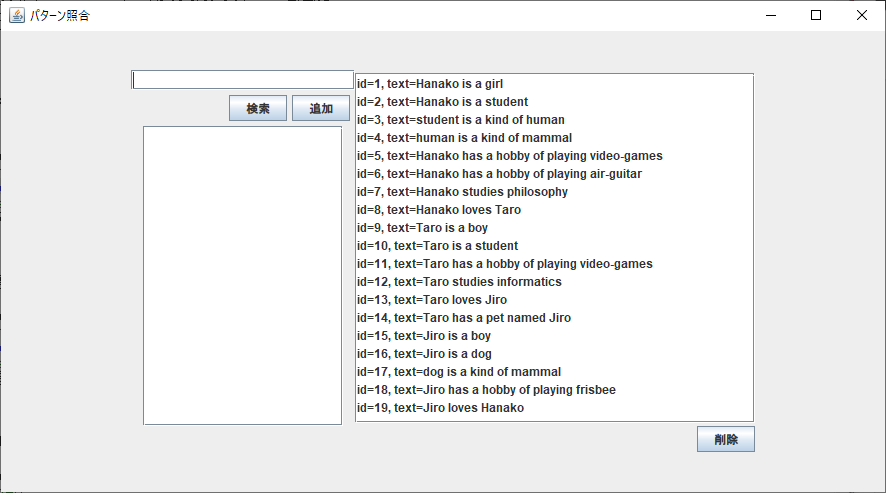
\includegraphics[scale=0.60]{images/scs2-3-1.png}
	\end{center}
  	\caption{初期状態}
\end{figure}
\clearpage

Matchingに関する質問文「?x has a hobby of playing video-games」を入力し,検索ボタンを押したところ,下図のような画面が得られる.

\begin{figure}[!hbt]
  	\begin{center}
  		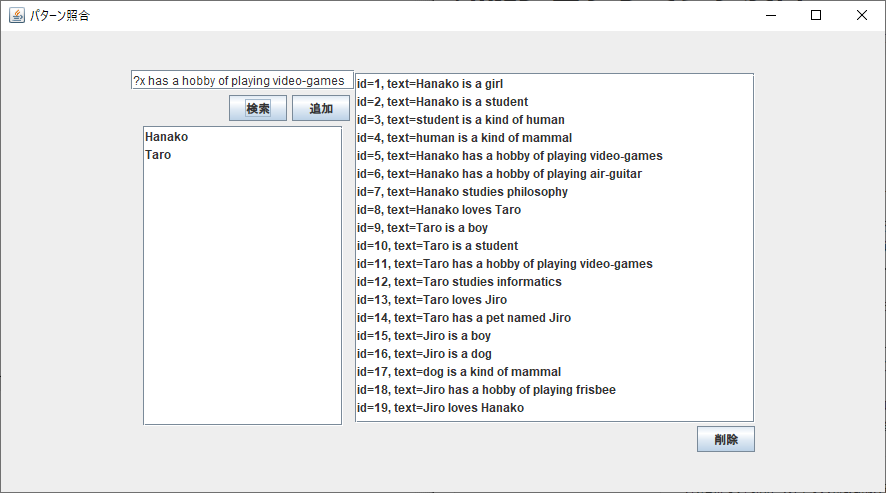
\includegraphics[scale=0.60]{images/scs2-3-2.png}
	\end{center}
  	\caption{Matchingの検索}
\end{figure}
\clearpage

\if0
Unifyに関する質問文「?x is a boy,?x loves ?y」を入力し,検索ボタンを押したところ,下図のような画面が得られる.

\begin{figure}[!hbt]
  	\begin{center}
  		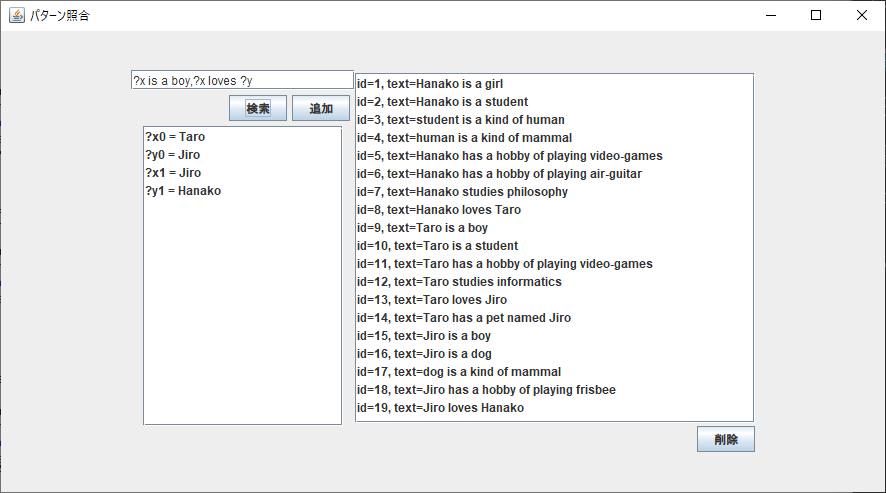
\includegraphics[scale=0.60]{images/scs2-3-6.png}
	\end{center}
  	\caption{Unifyの検索}
\end{figure}
\clearpage
\fi

データ「Shuhei is a boy」を入力し,追加ボタンを押したところ,下図のような画面が得られる.

\begin{figure}[!hbt]
  	\begin{center}
  		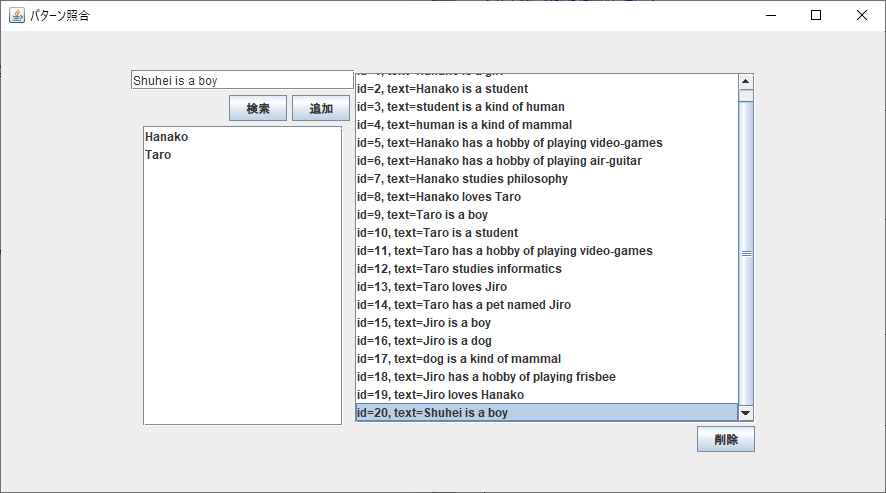
\includegraphics[scale=0.60]{images/scs2-3-3.png}
	\end{center}
  	\caption{データの追加}
\end{figure}
\clearpage

右のリストから「id=19,text=Jiro loves Hanako」を選択し,削除ボタンを押したところ,下図のような画面が得られる.

\begin{figure}[!hbt]
  	\begin{center}
  		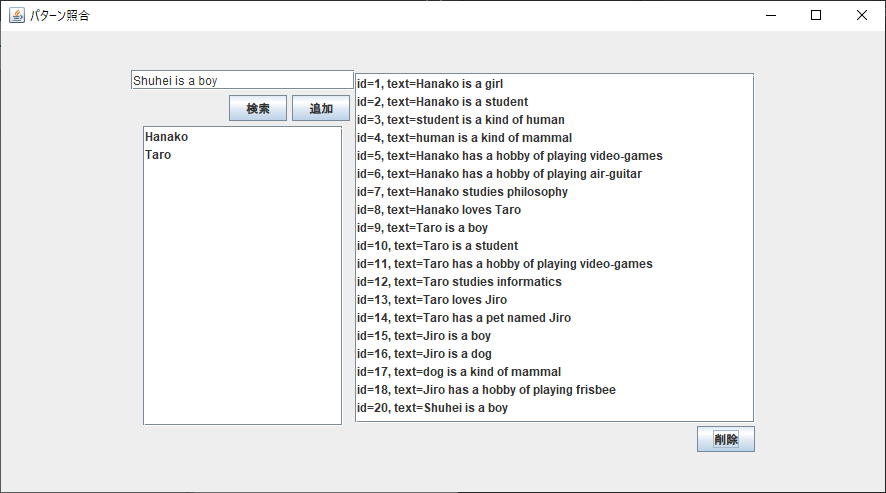
\includegraphics[scale=0.60]{images/scs2-3-4.png}
	\end{center}
  	\caption{データの削除}
\end{figure}
\clearpage

右上の×からプログラムを終了し,再度UnifyGUIを実行して起動したところ,下図のような画面が得られ,前回の追加・削除したデータが保持されていることが分かる.

\begin{figure}[!hbt]
  	\begin{center}
  		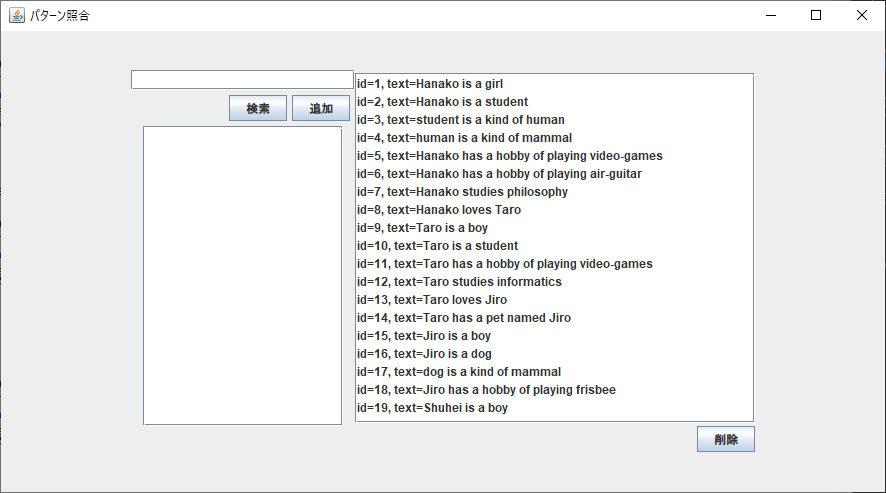
\includegraphics[scale=0.60]{images/scs2-3-5.png}
	\end{center}
  	\caption{プログラムの再起動}
\end{figure}
\clearpage

\subsection{考察}
ViewInterfaceを実装するためのクラスとしてViewクラスを別に作ったが,これによりPretenderからの値をUnifyGUIで使えるようになっただけでなく,UnifyGUIクラスを介さずともPresenterクラスを利用できるようになったため,結果として独立したクラスでViewInterfaceを実装してよかったと考えられる.

windowClosing  windowClosedはウィンドウがクローズされたときに呼び出される 強制終了は...

レイアウト大変だった

Paneいろいろあるんやな

グループ分担大変だった




\section{感想}

\end{document}